% ============================================================================
% sec4_diagnosis.tex — Where current methods fail (§4, W1 rev2; trimmed in-section)
% Target: ~570 words + Fig.2 (single column). Numbers only from plan 附B (B15-B24).
% ============================================================================
\section{Where Current Methods Fail on Filmed Glass}
\label{sec:diagnosis}

\begin{figure}[t]
\centering
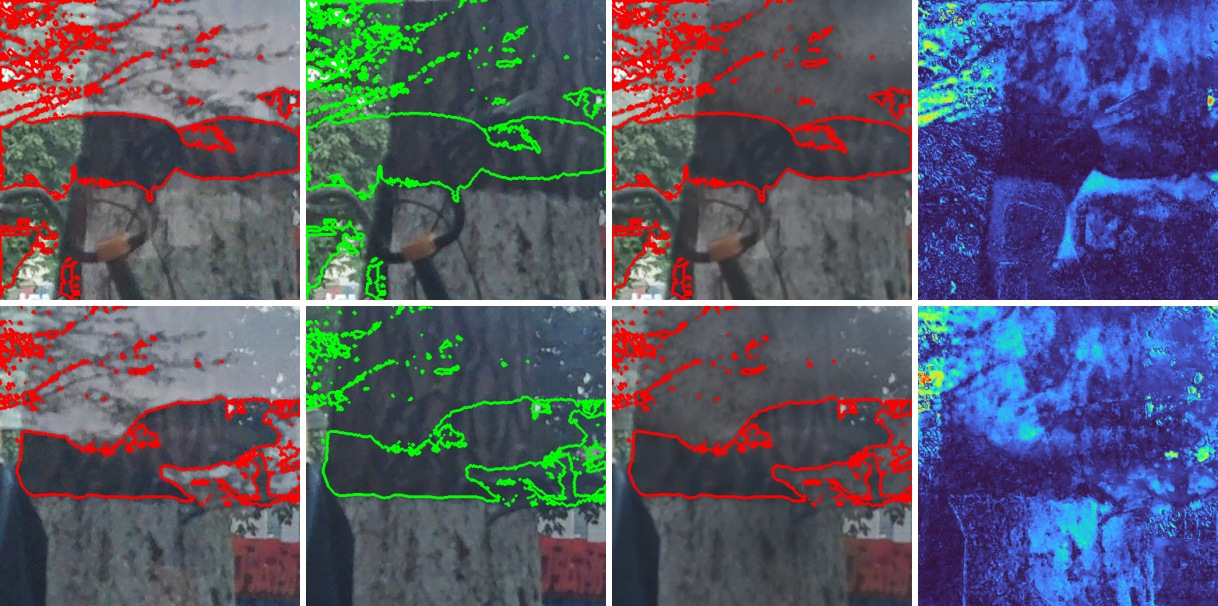
\includegraphics[width=\columnwidth]{fig/qual_omega.jpg}
\caption{\textbf{Where the damage happens.} Two development-panel scenes (rows):
input, ground truth, prediction and per-image-normalised absolute error. Contours mark
the hand-annotated occluder region; the error lights up along it rather than inside the
reflected content.}
\label{fig:qual}
\end{figure}

\subsection{The occluder region needs almost no change; its neighbourhood does}
\label{sec:axis1}

Partitioning each development-panel frame into the hand-annotated occluder region $\Om$,
a $15$\,px annulus around it and the far field gives three very different bands. Inside
$\Om$ the mean reflection magnitude $\mathbb{E}|I-T|$ is only $10.3$ gray levels, and
identity scores $24.52$\,dB, higher than any method in our baseline comparison: almost
nothing needs to change there. The annulus covers $44.4\%$ of the frame and its
$\mathbb{E}|I-T|$ is $44.4$ gray levels, $4.3\times$ that inside $\Om$ and $2.6\times$
that of the far field ($16.8$); identity scores $13.76$\,dB there. The far field lies
in between ($19.52$ identity). The aggregate signature: each of the baselines we tested scores below
identity inside $\Om$ ($\Om$-restricted PSNR $20.89$--$23.55$\,dB against $24.52$, i.e.\
all $\Delta_\Om<0$), and each is at its absolute worst in the annulus ($19.4$--$19.8$\,dB
versus $23.5$ far away). The consequence is perceptual: the annulus abuts an almost correct region, so its
residual is read as a \emph{boundary}; repairing it needs extrapolation from elsewhere in
the frame along semantic continuations rather than more reflection removal.

\subsection{The damage is structural, not photometric}
\label{sec:structural}

A photometric explanation would predict that models merely mis-scale $\Om$; they do not.
Restricting to $\Om$ and allowing a per-image affine correction before scoring, the
structure retained relative to ground truth is $1.14$ for identity, only $0.50$ for the
fine-tuned baseline and $0.65$ with the regularizer (development measurements;
affine-corrected MAE $10.51$, $12.82$, $11.70$ gray levels). We can also bound any content-agnostic method: a Gaussian smoothing
of the input is the best one can do without knowing the content. On the weakly reflected
$59\%$ of $\Om$ that ceiling is $29.50$\,dB against identity's $31.45$ and the
regularizer's $27.18$; on the strongly reflected $7\%$ it is $15.24$\,dB against $14.46$
and $13.48$. None of the models we trained beats a plain blur in either regime. The
remaining photometric head-room is per-image: a per-image affine oracle recovers
$0.15$--$0.26$\,dB whereas a shared leave-one-scene-out affine recovers $0.07$\,dB
(details in the supplementary material).

\subsection{Reflection and scene share the frequency band}
\label{sec:band}

$34.5\%$ of the reflection energy lies above a $\sigma{=}8$ low-pass, so it is not a veil
that can be filtered away. Replacing the low frequencies of a model output by the model's
own and the high frequencies by those of the \emph{input},
$\That'=\mathrm{LP}_\sigma(\That)+(I-\mathrm{LP}_\sigma(I))$, restores structure inside
$\Om$ but \emph{lowers} PSNR: from $22.26$ to $22.04$ and $21.66$\,dB at $\sigma{=}2,4$
(regularized model), and from $23.73$ to $23.39$ and $22.97$\,dB for a $50{:}50$
mixture. The band carrying the missing structure also carries the reflection.

\subsection{The load-bearing term is not about the region}
\label{sec:axis3}

Our objective contains a region-relative error inside $\Om$,
\begin{equation}
\reg=\lambda_{\Om}\,\mathbb{E}_{\Om}\!\left[\frac{|T-\That|}{\mathbb{E}_{\Om}|T-I|}\right],
\label{eq:lom}
\end{equation}
Removing it is catastrophic in a single-seed, pre-unified development ablation: the
panel score falls from $22.49$ to $18.33$\,dB, below identity's $18.44$\,dB (these are
historical numbers, not results of the unified protocol). Its power, however, is not the annotation. Replacing the hand mask by an
equal-area random disk, three seeds on a separate $82$-pair pool, gives $19.90\pm0.16$\,dB
against $19.41\pm0.54$ for the annotated region and $17.76\pm0.16$ for no region:
real-minus-random is $-0.49$\,dB (positive on one of three seeds). A whole-image relative
error without any region reaches $20.05$\,dB and a fixed per-pair disk $20.25\pm0.29$\,dB.
What matters is thus \emph{that a compact region is supervised with a relative
normalization}, not that it is the occluder region; a per-pixel version needs no mask,
which we test as a controlled intervention (Sec.~\ref{sec:method}).
